\Gls{ml} has become an important sub-field of computer science. It emulates human-like learning using mathematical models, so predictions can be made about new data in the future. Rather than explicitly programming how to make those predictions, the developer feeds sample data to the model during \textit{training}. Once the accuracy of the trained model is sufficient, it can be used for \textit{inference}. The model can be thought of as the approximation of a function mapping from the input data to some output, e.g., a label for classification, or a numerical value for regression~\cite[p.~164]{IanGoodfellow.2016}.

\section{Artificial Neural Networks}
While there are a variety of \gls{ml} models in use today, \glspl{ann} are among the most powerful and flexible, due to their ability to represent complex functions~\cite[p.~163]{IanGoodfellow.2016}. They find application in fields as diverse as image and speech recognition, movie recommendations and medical diagnosis.

\Glspl{ann} are composed of multiple layers, with the output of one layer being the input of another layer. The first layer receives the input data, and the last layer produces the final output. With an increasing number of layers, or \textit{depth} of the network, more complex functions can be approximated. All layers perform some computation given a set of trained or specified parameters and the input. Both parameters and inputs are tensors, a higher-dimensional generalization of vectors and matrices. Traditional \glspl{ann} feature only fully-connected layers with some activation function.

Grid-like data such as time series (1D) or images (2D) benefit from additional layers found in \glspl{cnn}~\cite[p.~326]{IanGoodfellow.2016}. \Glspl{cnn} apply convolution and pooling to a region of the input tensor in a sliding fashion, so entries only interact with other entries in their neighborhood. Convolution applies one or more kernels to the input, which are element-wise multiplied with the current region and then summed up into a single output value. Pooling averages or finds the maximum of the region as output value. Both operations support a variable stride and padding. \Glspl{cnn} are an important tool in state-of-the-art computer vision applications.

While neural network models logically consist of a series of layers, machine learning frameworks usually represent them in a computation graph. The computation graph's first vertex is the input node, followed by a number of tensor operators performing the layer's computation, and finally an output node. The edges describes how data flows between the vertices.

\section{Inference Optimization}
Typically, the amount of inferences heavily outweighs the amount of trainings, since training only needs to be done once (albeit model re-training is usually done periodically when new training data is available). For this reason, while training takes longer by several orders of magnitude, speeding up inference has a larger impact and is an important field. 
Reduction of the inference time has a number of advantages:
\begin{itemize}
	\item less hardware is required to achieve the same inference rate
	\item higher inference rate can be achieved with same hardware
	\item real-time applications are made possible, e.g., autonomous driving, industrial monitoring
\end{itemize}
In real-time applications with a high inference rate, even small improvements in inference performance (in the order of milliseconds) can be critical to guarantee the required throughput.
For example, a major hard drive manufacturer detects defects in their products using a \gls{cnn}-based smart manufacturing solution~\cite[p.~11]{LyveDataLabs.2019}. They perform inference on 3 million images every day, so if they could only save \SI{5}{\milli\second} per image due to some optimization, they could save over \SI{4}{\hour} every day~\cite{Seagate.2019}. Alternatively, they could save costs by needing less servers that are equipped with expensive accelerator devices.

Accelerator devices such as \glspl{gpu}, tensor processing units or field-programmable gate arrays are used to speed up both training and inference. Every device has different features such as specialized instructions, memory size and layout, cache access, and parallelization support. However, generic models cannot make full use of accelerator capabilities and fall short of leveraging the full potential. Consequently, models need to be attuned to the \gls{targetdevice} to achieve the best inference performance. But even if no special accelerator devices are used but only a conventional CPU, adapting to the specific architecture can yield great performance benefits~\cite[p.~1]{Liu.2019}. In the traditional machine workflow, the trained model is deployed as-is(Figure \ref{fig:ml-workflow-old}). Inference optimization adds an additional step, turning the trained model into a functionally equivalent but optimized version for inference (Figure \ref{fig:ml-workflow-new}). In this step, we first apply high-level transformations that rewrite the computation graph by fusing tensor operators, pre-computing constant parts or transforming the data layout in memory~\cites[p.~1--3]{Chen.2018b}. More importantly, however, we can change the low-level implementation of tensor operators.

\begin{figure}
	\begin{minipage}[b]{.5\textwidth}
		\centering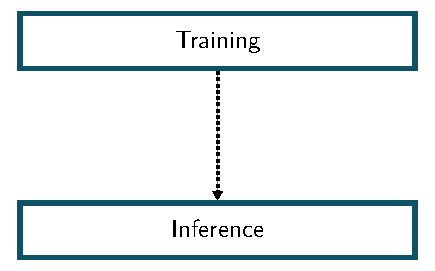
\includegraphics{ml_workflow_1.pdf}
		\subcaption{Traditional without inference optimization}\label{fig:ml-workflow-old}
	\end{minipage}%
	\begin{minipage}[b]{.5\textwidth}
		\centering\includegraphics{ml_workflow_2.pdf}
		\subcaption{Improved with inference optimization}\label{fig:ml-workflow-new}
	\end{minipage}
	\caption[Traditional vs. optimized machine learning workflow]{Machine learning workflow}
	\label{fig:ml-workflow}
\end{figure}

Convolution operations are computationally very intensive and make up the majority of state-of-the-art \glspl{cnn}, such as Inception\cite{Szegedy.2015} and ResNet\cite{He.2015}. Therefore, tensor operator optimization should focus on convolution over other types like pooling and fully-connected. It is not possible to optimize convolutions in general, but we need to optimize for every distinct parameter set that is present in the computation graph, i.e. combination of input shape, kernel shape, padding, and stride. This means that the effort increases with a higher variety of layer configurations.

The model determines what should be calculated, but it does not specify how it is calculated. The actual implementation offers lots of optimization potential. There is always a generic default implementation which is the straightforward way of performing the calculation. However, it does not consider shared memory between threads or cache access patterns, which can have a significant adverse effect on performance~\cite{Hu.2017}. Techniques such as loop unrolling, reordering and tiling as well as multi-dimensional threading and tensor compute instructions can help leverage the accelerator's capabilities, but there is an abundance of combinations of tiling sizes, loop unrolling factors and thread numbers, any of which could be the best one but is very much specific to the target device~\cite[p.~2]{Chen.2018b}. Finding the optimal such combination is the goal of inference performance optimization.

\section{Manual Optimization}
state of the art cuDNN and TensorRT and Intel MKL, taken as baseline
requires deep knowledge of target device, usually provided by vendor
limitations
- no support for new devices
- no support for unconventional shapes
- no support for new graph-level optimizations
elaborate limitations
high-level optimization need to wait until vendor provides low-level support


\section{Automated Optimization}
vendor-agnostic and does not require expert knowledge
Enables innovation by enabling high-level optimization and fostering experimentation with unconventional layers, not supported by manual frameworks
describe autotuning process on high level
definition of search space (loop unrolling, tiling, threads)
Problem: search space is very large (billions), and any one of them could be the best one for one target device

impossible to try all
autotuning frameworks have some solution to explore search space rapidly
look at TVM and TC

has same or even better performance than hand-optimized libraries
show numbers

There are two frameworks that implement autotuning

\subsection{TensorComprehensions}
does not use machine learning

\subsection{TVM}
using machine learning
TVM is framework that proposed and implements autotuning

import from many frontends, compilation for many backends
has own graph-level and tensor operator-level representation
calls target-specific compiler

define autotuning job, task
first extraction of tasks
schedules as abstraction with knobs
details of autotuning process
Profiling repeated multiple times
RPC allows autotuning logic to run on powerful server, but profiling to happen on target device
with figure

In this project, we use TVM because of the novel, machine learning-based approach
Using (commit id) with a few modifications to support measurements (check what else we changed)
